% !TeX spellcheck = es_ES
\chapter{Solución propuesta}
\label{ch:chap03}

\section{Alcance y objetivos}
\label{sec:alcance}

Este proyecto se centra en la implementación completa de una aplicación capaz de calcular tanto la matriz de factores de forma como el vector de radiosidad final. Se agrega especial énfasis en la comparación del rendimiento de los distintos métodos en la Sección \ref{ch:chap02} para escenas compuestas por triángulos y cuadriláteros.

Se propone comparar cuatro métodos para el cálculo de factores de forma:

\begin{enumerate}
 	\item Cálculo de factores de forma utilizando el hemi-cubo
 	\item  Cálculo de factores de forma utilizando trazado de rayos
 	\item Cálculo de factores de forma extendidos utilizando rasterización
 	\item Cálculo de factores  de forma extendidos utilizando trazado de rayos
\end{enumerate}

Además, se propone implementar una interfaz de usuario que facilite la carga, edición y visualización de los objetos que componen la escena y sus respectivas propiedades (geometría, emisión inicial, coeficientes de reflexión difusa y especular, y radiosidad).

\section{Proceso de desarrollo}
\label{sec:procdes}

Dada la naturaleza del proyecto, es deseable establecer una metodología de desarrollo para facilitar el proceso de seguimiento del progreso incluso cuando el equipo de desarrollo fue compuesto por un único integrante.

Para ello, internamente, se utilizó una metodología ágil de desarrollo similar a la conocida como \textit{Kanban}.

Los principios claves del método aplicado a este proyecto fueron:
\begin{itemize}
	\item La visualización sencilla del curso de trabajo (una lista de tareas a realizar conocida como \textit{Backlog})
	\item La limitación de las tareas en progreso con el objetivo de eliminar la sobrecarga de trabajo.
	\item Dirigir y gestionar el flujo de trabajo implica la priorización de tareas a realizar dada una cantidad finita de recursos.
\end{itemize}

La gestión de las tareas a realizar se llevó a cabo en el repositorio del proyecto, con tareas como las vistas en la Figura \ref{img:kanban}, donde se consideran un conjunto de tareas:

\begin{itemize}
	\item Backlog: Las tareas a realizar, en orden de importancia.
	\item In progress: Las tareas actualmente en desarrollo.
	\item Done: Las tareas cuya funcionalidad fue completamente desarrollada y probada.
\end{itemize}

\vspace{5mm}
\begin{minipage}[h]{0.8\linewidth}
	\centering
	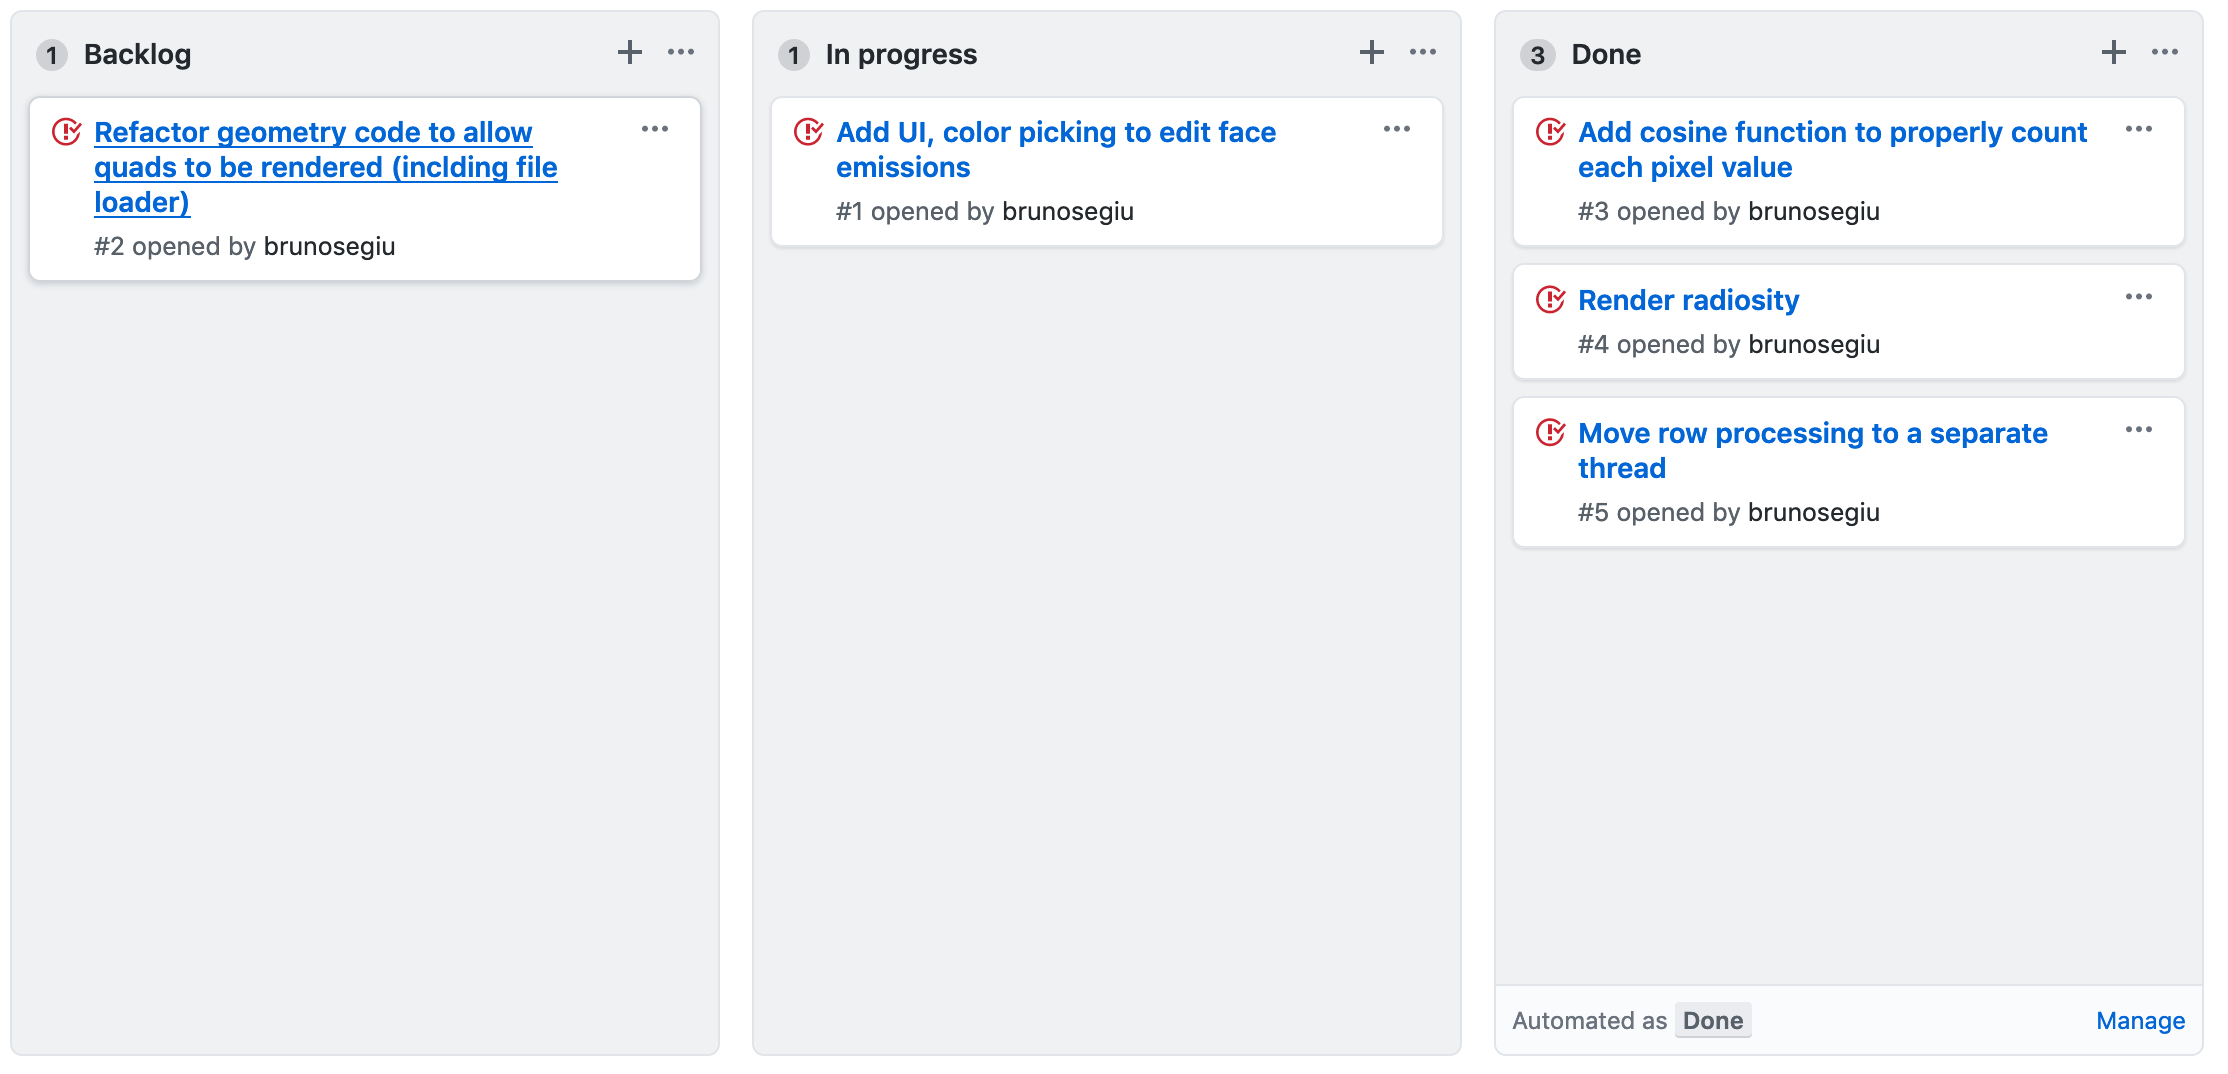
\includegraphics[width=\linewidth]{assets/kanban}
	\captionof{figure}{Tabla de Kanban utilizada en el proyecto}
	\label{img:kanban}
\end{minipage}

\section{Diseño}
\label{sec:disenio}

Con la finalidad de evitar el alto acoplamiento, facilitar la extensión y reducir la cantidad de errores de integración se tomó la decisión de utilizar distintos módulos y sub-módulos que ofrezcan un conjunto de funcionalidades bien definido utilizando programación orientada a objetos. Esta decisión permite el añadido de nuevas características y la optimización de ciertas funcionalidades independientemente de los demás módulos construidos.

El diseño de la solución comprende dos componentes principales, la interfaz gráfica de usuario (GUI, por su nombre en inglés) y el motor de renderizado.

\subsection{Motor de renderizado}
\label{sec:engine}

El paquete del motor de renderizado se compone de un conjunto de sub-módulos, el primero de ellos que maneja el pre-procesado de una escena, es decir, el cálculo de la matriz de factores de forma y la radiosidad. El siguiente conjunto de sub-módulos se ocupan del renderizado en tiempo real de la escena, así como la carga de modelos desde el disco duro, la modificación de materiales, entre otras funcionalidades detalladas en \ref{sec:ui}.

\subsubsection{Módulo de geometría}

El módulo de geometría encapsula la información de las escenas leídas desde el disco duro, además de adaptar y optimizar los formatos de las primitivas geométricas para ser utilizados en las APIs de dibujado de terceros. La clase \verb|Scene|, diagramada en la Figura \ref{img:geom}, carga distintos objetos desde el disco duro que son manejados como una instancia de \verb|Mesh|.


\vspace{5mm}
\begin{minipage}[h]{0.7\linewidth}
	\centering
	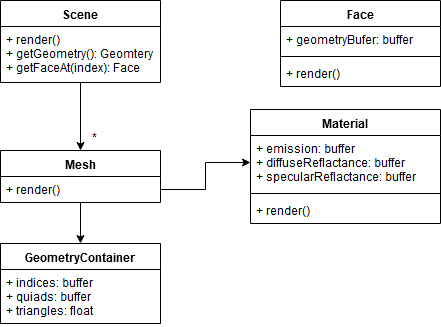
\includegraphics[width=\linewidth]{assets/geometry}
	\captionof{figure}{Módulo de manejo de geometría}
	\label{img:geom}
\end{minipage}

\subsubsection{Módulo de pre-procesado}

El módulo de preprocesado se compone de un controlador principal (\verb|PreprocessController| en la figura \ref{img:procesado}), que maneja el estado y la ejecución de  los comandos de los distintos \textit{pipelines} implementados que resuelven el cálculo de la radiosidad.

\vspace{5mm}
\begin{minipage}[h]{\linewidth}
	\centering
	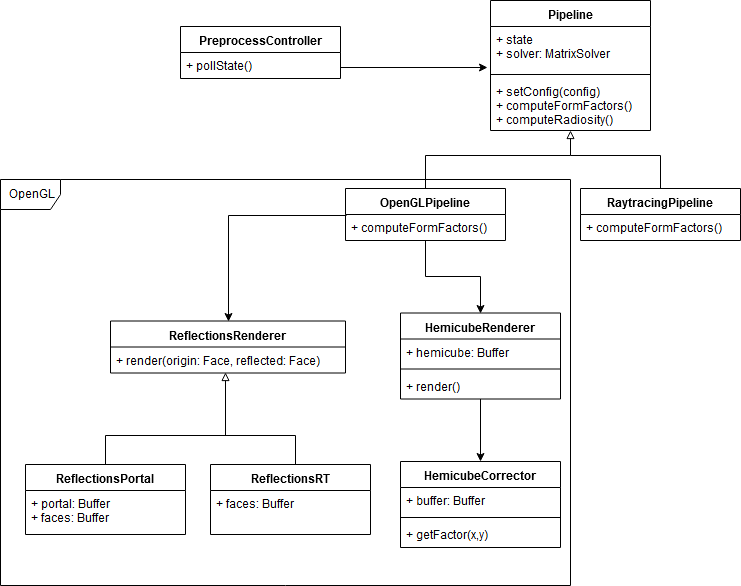
\includegraphics[width=\linewidth]{assets/preprocess}
	\captionof{figure}{Arquitectura del módulo de pre-procesado}
	\label{img:procesado}
\end{minipage}


La clase Pipeline y sus derivadas de rasterización y traza de rayos definen un conjunto de tareas que se realizarán para calcular los factores de forma y el vector de radiosdiad. Las tareas suponen incializar el pipeline con información de la escena, calcular los factores de forma (eventualmente considerando la reflexión especular) y calcular el vector de radiosidad para los parches de la escena.
Por ello, una instancia del pipeline es definida a partir de un conjunto de funciones ejecutadas en el siguiente orden:

\begin{enumerate}
	\item \verb|setConfig(scene, intrp, ref, chan, sol)|
	\item \verb|computeFormFactors()|
	\item \verb|computeRadiosity()|
\end{enumerate}

La función \verb|computeFormFactors()| variará dependiendo del método de cálculo elegido (Figura \ref{img:procesado}), donde puede utilizarse el método del hemi-cubo o el de raytracing. El primero de ellos utilizará un \textit{pipeline} configurado utilizando una API de rasterización, mientras que el segundo utilizará una API capaz de calcular intersecciones utilizando rayos.

La ejecución de \verb|computeRadiosity()| dependerá directamente del manejador \verb|Solver| seleccionado por el usuario, este último ejecutará el algoritmo que calculará el vector de radiosidades para la escena, resolviendo el sistema lineal de radiosidad.

\subsubsection{Módulo de visualización}

El módulo de visualización se encarga de renderizar la escena actual desde el punto de vista seleccionado por el usuario. Además, debe tener la capacidad de mostrar las distintas propiedades de los materiales, tales como valor de emisión inicial, valor de reflexión especular y, visualización de geometría, para así facilitar la edición de las propiedades de los objetos y de sus caras. El proceso de renderizado comienza con una instancia de la clase \verb|DisplayController| que dibuja un conjunto de imágenes correspondiente a las propiedades de los materiales, \verb|SceneRenderer| en la Figura \ref{img:vis}. Luego un dibujante de texturas \verb|TextureRenderer| selecciona y convierte correctamente el resultado anterior a valores de tres canales (RGB). El módulo de visualización siempre toma una textura bidimensional como parámetro de salida.

\vspace{5mm}
\begin{minipage}[h]{0.8\linewidth}
	\centering
	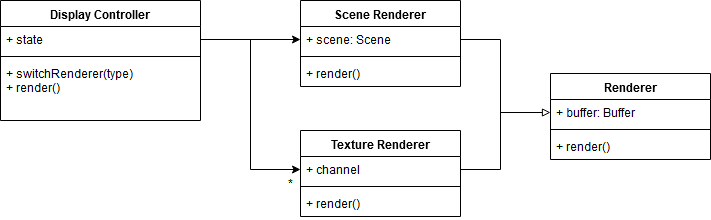
\includegraphics[width=\linewidth]{assets/display}
	\captionof{figure}{Arquitectura del módulo de visualización}
	\label{img:vis}
\end{minipage}

\subsection{Interfaz gráfica}

El módulo de visualización (UI) utiliza una arquitectura basada en el paradigma del bucle de eventos (Figura \ref{img:ui}), consiste en un bucle que detecta y maneja los distintos eventos recibidos por el sistema. Este método es útil para el manejo sencillo de la concurrencia en sistemas con múltiples hilos en ejecución, y es de fácil implementación pues procesa cada uno de los eventos completamente antes de procesar el siguiente.

 El  \textit{bucle de eventos} procesa todos los eventos de la aplicación, lo que desencadena un conjunto de acciones que modifican su estado de la interfaz de usuario. Este estado es dibujado por un conjunto de componentes, que no son más que presentadores del estado actual. Es decir, a partir de un conjunto de valores los presentan en un formato gráfico adecuado y sencillo de comprender.

\vspace{5mm}
\begin{minipage}[h]{0.8\linewidth}
	\centering
	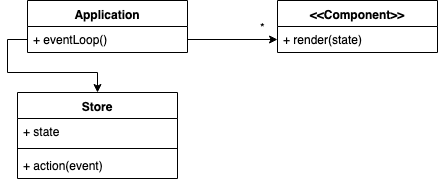
\includegraphics[width=\linewidth]{assets/ui}
	\captionof{figure}{Arquitectura general del módulo de interfaz de usuario}
	\label{img:ui}
\end{minipage}

\label{sec:ui}